% Created by tikzDevice version 0.12.3.1 on 2023-05-05 12:22:58
% !TEX encoding = UTF-8 Unicode
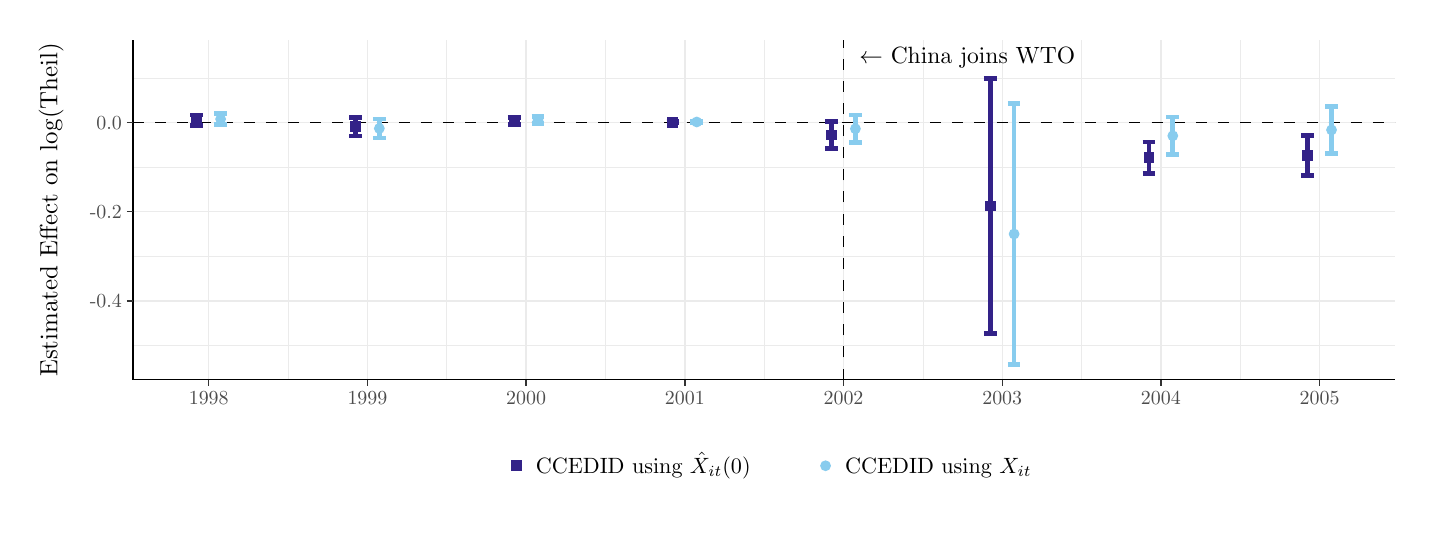
\begin{tikzpicture}[x=1pt,y=1pt]
\definecolor{fillColor}{RGB}{255,255,255}
\path[use as bounding box,fill=fillColor] (0,0) rectangle (498.66,174.53);
\begin{scope}
\path[clip] (  0.00,  0.00) rectangle (498.66,174.53);
\definecolor{drawColor}{RGB}{255,255,255}

\path[draw=drawColor,line width= 0.5pt,line join=round,line cap=round,fill=fillColor] ( -0.00,  0.00) rectangle (498.66,174.53);
\end{scope}
\begin{scope}
\path[clip] ( 38.10, 47.36) rectangle (494.16,170.03);
\definecolor{fillColor}{RGB}{255,255,255}

\path[fill=fillColor] ( 38.10, 47.36) rectangle (494.16,170.03);
\definecolor{drawColor}{gray}{0.92}

\path[draw=drawColor,line width= 0.2pt,line join=round] ( 38.10, 59.72) --
	(494.16, 59.72);

\path[draw=drawColor,line width= 0.2pt,line join=round] ( 38.10, 91.94) --
	(494.16, 91.94);

\path[draw=drawColor,line width= 0.2pt,line join=round] ( 38.10,124.17) --
	(494.16,124.17);

\path[draw=drawColor,line width= 0.2pt,line join=round] ( 38.10,156.40) --
	(494.16,156.40);

\path[draw=drawColor,line width= 0.2pt,line join=round] ( 94.09, 47.36) --
	( 94.09,170.03);

\path[draw=drawColor,line width= 0.2pt,line join=round] (151.44, 47.36) --
	(151.44,170.03);

\path[draw=drawColor,line width= 0.2pt,line join=round] (208.78, 47.36) --
	(208.78,170.03);

\path[draw=drawColor,line width= 0.2pt,line join=round] (266.13, 47.36) --
	(266.13,170.03);

\path[draw=drawColor,line width= 0.2pt,line join=round] (323.47, 47.36) --
	(323.47,170.03);

\path[draw=drawColor,line width= 0.2pt,line join=round] (380.82, 47.36) --
	(380.82,170.03);

\path[draw=drawColor,line width= 0.2pt,line join=round] (438.17, 47.36) --
	(438.17,170.03);

\path[draw=drawColor,line width= 0.5pt,line join=round] ( 38.10, 75.83) --
	(494.16, 75.83);

\path[draw=drawColor,line width= 0.5pt,line join=round] ( 38.10,108.06) --
	(494.16,108.06);

\path[draw=drawColor,line width= 0.5pt,line join=round] ( 38.10,140.29) --
	(494.16,140.29);

\path[draw=drawColor,line width= 0.5pt,line join=round] ( 65.42, 47.36) --
	( 65.42,170.03);

\path[draw=drawColor,line width= 0.5pt,line join=round] (122.77, 47.36) --
	(122.77,170.03);

\path[draw=drawColor,line width= 0.5pt,line join=round] (180.11, 47.36) --
	(180.11,170.03);

\path[draw=drawColor,line width= 0.5pt,line join=round] (237.46, 47.36) --
	(237.46,170.03);

\path[draw=drawColor,line width= 0.5pt,line join=round] (294.80, 47.36) --
	(294.80,170.03);

\path[draw=drawColor,line width= 0.5pt,line join=round] (352.15, 47.36) --
	(352.15,170.03);

\path[draw=drawColor,line width= 0.5pt,line join=round] (409.49, 47.36) --
	(409.49,170.03);

\path[draw=drawColor,line width= 0.5pt,line join=round] (466.84, 47.36) --
	(466.84,170.03);
\definecolor{drawColor}{RGB}{0,0,0}

\path[draw=drawColor,line width= 0.6pt,dash pattern=on 4pt off 4pt ,line join=round] ( 38.10,140.29) -- (494.16,140.29);

\path[draw=drawColor,line width= 0.6pt,dash pattern=on 4pt off 4pt ,line join=round] (294.80, 47.36) -- (294.80,170.03);

\node[text=drawColor,anchor=base west,inner sep=0pt, outer sep=0pt, scale=  0.85] at (300.54,161.52) {$\leftarrow$ China joins WTO};
\definecolor{drawColor}{RGB}{51,34,136}

\path[draw=drawColor,line width= 1.7pt,line join=round] ( 58.83,143.01) --
	( 63.41,143.01);

\path[draw=drawColor,line width= 1.7pt,line join=round] ( 61.12,143.01) --
	( 61.12,139.26);

\path[draw=drawColor,line width= 1.7pt,line join=round] ( 58.83,139.26) --
	( 63.41,139.26);

\path[draw=drawColor,line width= 1.7pt,line join=round] (116.17,142.13) --
	(120.76,142.13);

\path[draw=drawColor,line width= 1.7pt,line join=round] (118.46,142.13) --
	(118.46,135.35);

\path[draw=drawColor,line width= 1.7pt,line join=round] (116.17,135.35) --
	(120.76,135.35);

\path[draw=drawColor,line width= 1.7pt,line join=round] (173.52,142.12) --
	(178.10,142.12);

\path[draw=drawColor,line width= 1.7pt,line join=round] (175.81,142.12) --
	(175.81,139.60);

\path[draw=drawColor,line width= 1.7pt,line join=round] (173.52,139.60) --
	(178.10,139.60);

\path[draw=drawColor,line width= 1.7pt,line join=round] (230.86,140.66) --
	(235.45,140.66);

\path[draw=drawColor,line width= 1.7pt,line join=round] (233.16,140.66) --
	(233.16,140.15);

\path[draw=drawColor,line width= 1.7pt,line join=round] (230.86,140.15) --
	(235.45,140.15);

\path[draw=drawColor,line width= 1.7pt,line join=round] (288.21,140.68) --
	(292.79,140.68);

\path[draw=drawColor,line width= 1.7pt,line join=round] (290.50,140.68) --
	(290.50,130.85);

\path[draw=drawColor,line width= 1.7pt,line join=round] (288.21,130.85) --
	(292.79,130.85);

\path[draw=drawColor,line width= 1.7pt,line join=round] (345.55,156.17) --
	(350.14,156.17);

\path[draw=drawColor,line width= 1.7pt,line join=round] (347.85,156.17) --
	(347.85, 64.02);

\path[draw=drawColor,line width= 1.7pt,line join=round] (345.55, 64.02) --
	(350.14, 64.02);

\path[draw=drawColor,line width= 1.7pt,line join=round] (402.90,133.24) --
	(407.49,133.24);

\path[draw=drawColor,line width= 1.7pt,line join=round] (405.19,133.24) --
	(405.19,121.75);

\path[draw=drawColor,line width= 1.7pt,line join=round] (402.90,121.75) --
	(407.49,121.75);

\path[draw=drawColor,line width= 1.7pt,line join=round] (460.24,135.46) --
	(464.83,135.46);

\path[draw=drawColor,line width= 1.7pt,line join=round] (462.54,135.46) --
	(462.54,120.99);

\path[draw=drawColor,line width= 1.7pt,line join=round] (460.24,120.99) --
	(464.83,120.99);
\definecolor{drawColor}{RGB}{136,204,238}

\path[draw=drawColor,line width= 1.7pt,line join=round] ( 67.43,143.39) --
	( 72.01,143.39);

\path[draw=drawColor,line width= 1.7pt,line join=round] ( 69.72,143.39) --
	( 69.72,139.59);

\path[draw=drawColor,line width= 1.7pt,line join=round] ( 67.43,139.59) --
	( 72.01,139.59);

\path[draw=drawColor,line width= 1.7pt,line join=round] (124.77,141.54) --
	(129.36,141.54);

\path[draw=drawColor,line width= 1.7pt,line join=round] (127.07,141.54) --
	(127.07,134.67);

\path[draw=drawColor,line width= 1.7pt,line join=round] (124.77,134.67) --
	(129.36,134.67);

\path[draw=drawColor,line width= 1.7pt,line join=round] (182.12,142.37) --
	(186.71,142.37);

\path[draw=drawColor,line width= 1.7pt,line join=round] (184.41,142.37) --
	(184.41,139.82);

\path[draw=drawColor,line width= 1.7pt,line join=round] (182.12,139.82) --
	(186.71,139.82);

\path[draw=drawColor,line width= 1.7pt,line join=round] (239.46,140.71) --
	(244.05,140.71);

\path[draw=drawColor,line width= 1.7pt,line join=round] (241.76,140.71) --
	(241.76,140.19);

\path[draw=drawColor,line width= 1.7pt,line join=round] (239.46,140.19) --
	(244.05,140.19);

\path[draw=drawColor,line width= 1.7pt,line join=round] (296.81,142.94) --
	(301.40,142.94);

\path[draw=drawColor,line width= 1.7pt,line join=round] (299.10,142.94) --
	(299.10,133.06);

\path[draw=drawColor,line width= 1.7pt,line join=round] (296.81,133.06) --
	(301.40,133.06);

\path[draw=drawColor,line width= 1.7pt,line join=round] (354.15,147.02) --
	(358.74,147.02);

\path[draw=drawColor,line width= 1.7pt,line join=round] (356.45,147.02) --
	(356.45, 52.94);

\path[draw=drawColor,line width= 1.7pt,line join=round] (354.15, 52.94) --
	(358.74, 52.94);

\path[draw=drawColor,line width= 1.7pt,line join=round] (411.50,142.29) --
	(416.09,142.29);

\path[draw=drawColor,line width= 1.7pt,line join=round] (413.79,142.29) --
	(413.79,128.61);

\path[draw=drawColor,line width= 1.7pt,line join=round] (411.50,128.61) --
	(416.09,128.61);

\path[draw=drawColor,line width= 1.7pt,line join=round] (468.85,145.98) --
	(473.43,145.98);

\path[draw=drawColor,line width= 1.7pt,line join=round] (471.14,145.98) --
	(471.14,129.17);

\path[draw=drawColor,line width= 1.7pt,line join=round] (468.85,129.17) --
	(473.43,129.17);
\definecolor{fillColor}{RGB}{51,34,136}

\path[fill=fillColor] ( 59.16,139.18) --
	( 63.08,139.18) --
	( 63.08,143.10) --
	( 59.16,143.10) --
	cycle;

\path[fill=fillColor] (116.50,136.78) --
	(120.43,136.78) --
	(120.43,140.70) --
	(116.50,140.70) --
	cycle;

\path[fill=fillColor] (173.85,138.90) --
	(177.77,138.90) --
	(177.77,142.82) --
	(173.85,142.82) --
	cycle;

\path[fill=fillColor] (231.19,138.44) --
	(235.12,138.44) --
	(235.12,142.36) --
	(231.19,142.36) --
	cycle;

\path[fill=fillColor] (288.54,133.80) --
	(292.46,133.80) --
	(292.46,137.73) --
	(288.54,137.73) --
	cycle;

\path[fill=fillColor] (345.88,108.13) --
	(349.81,108.13) --
	(349.81,112.06) --
	(345.88,112.06) --
	cycle;

\path[fill=fillColor] (403.23,125.53) --
	(407.15,125.53) --
	(407.15,129.46) --
	(403.23,129.46) --
	cycle;

\path[fill=fillColor] (460.57,126.26) --
	(464.50,126.26) --
	(464.50,130.18) --
	(460.57,130.18) --
	cycle;
\definecolor{fillColor}{RGB}{136,204,238}

\path[fill=fillColor] ( 69.72,141.49) circle (  1.96);

\path[fill=fillColor] (127.07,138.11) circle (  1.96);

\path[fill=fillColor] (184.41,141.09) circle (  1.96);

\path[fill=fillColor] (241.76,140.45) circle (  1.96);

\path[fill=fillColor] (299.10,138.00) circle (  1.96);

\path[fill=fillColor] (356.45, 99.98) circle (  1.96);

\path[fill=fillColor] (413.79,135.45) circle (  1.96);

\path[fill=fillColor] (471.14,137.58) circle (  1.96);
\end{scope}
\begin{scope}
\path[clip] (  0.00,  0.00) rectangle (498.66,174.53);
\definecolor{drawColor}{RGB}{0,0,0}

\path[draw=drawColor,line width= 0.5pt,line join=round] ( 38.10, 47.36) --
	( 38.10,170.03);
\end{scope}
\begin{scope}
\path[clip] (  0.00,  0.00) rectangle (498.66,174.53);
\definecolor{drawColor}{gray}{0.30}

\node[text=drawColor,anchor=base east,inner sep=0pt, outer sep=0pt, scale=  0.72] at ( 34.05, 73.35) {-0.4};

\node[text=drawColor,anchor=base east,inner sep=0pt, outer sep=0pt, scale=  0.72] at ( 34.05,105.58) {-0.2};

\node[text=drawColor,anchor=base east,inner sep=0pt, outer sep=0pt, scale=  0.72] at ( 34.05,137.81) {0.0};
\end{scope}
\begin{scope}
\path[clip] (  0.00,  0.00) rectangle (498.66,174.53);
\definecolor{drawColor}{gray}{0.20}

\path[draw=drawColor,line width= 0.5pt,line join=round] ( 35.85, 75.83) --
	( 38.10, 75.83);

\path[draw=drawColor,line width= 0.5pt,line join=round] ( 35.85,108.06) --
	( 38.10,108.06);

\path[draw=drawColor,line width= 0.5pt,line join=round] ( 35.85,140.29) --
	( 38.10,140.29);
\end{scope}
\begin{scope}
\path[clip] (  0.00,  0.00) rectangle (498.66,174.53);
\definecolor{drawColor}{RGB}{0,0,0}

\path[draw=drawColor,line width= 0.5pt,line join=round] ( 38.10, 47.36) --
	(494.16, 47.36);
\end{scope}
\begin{scope}
\path[clip] (  0.00,  0.00) rectangle (498.66,174.53);
\definecolor{drawColor}{gray}{0.20}

\path[draw=drawColor,line width= 0.5pt,line join=round] ( 65.42, 45.11) --
	( 65.42, 47.36);

\path[draw=drawColor,line width= 0.5pt,line join=round] (122.77, 45.11) --
	(122.77, 47.36);

\path[draw=drawColor,line width= 0.5pt,line join=round] (180.11, 45.11) --
	(180.11, 47.36);

\path[draw=drawColor,line width= 0.5pt,line join=round] (237.46, 45.11) --
	(237.46, 47.36);

\path[draw=drawColor,line width= 0.5pt,line join=round] (294.80, 45.11) --
	(294.80, 47.36);

\path[draw=drawColor,line width= 0.5pt,line join=round] (352.15, 45.11) --
	(352.15, 47.36);

\path[draw=drawColor,line width= 0.5pt,line join=round] (409.49, 45.11) --
	(409.49, 47.36);

\path[draw=drawColor,line width= 0.5pt,line join=round] (466.84, 45.11) --
	(466.84, 47.36);
\end{scope}
\begin{scope}
\path[clip] (  0.00,  0.00) rectangle (498.66,174.53);
\definecolor{drawColor}{gray}{0.30}

\node[text=drawColor,anchor=base,inner sep=0pt, outer sep=0pt, scale=  0.72] at ( 65.42, 38.35) {1998};

\node[text=drawColor,anchor=base,inner sep=0pt, outer sep=0pt, scale=  0.72] at (122.77, 38.35) {1999};

\node[text=drawColor,anchor=base,inner sep=0pt, outer sep=0pt, scale=  0.72] at (180.11, 38.35) {2000};

\node[text=drawColor,anchor=base,inner sep=0pt, outer sep=0pt, scale=  0.72] at (237.46, 38.35) {2001};

\node[text=drawColor,anchor=base,inner sep=0pt, outer sep=0pt, scale=  0.72] at (294.80, 38.35) {2002};

\node[text=drawColor,anchor=base,inner sep=0pt, outer sep=0pt, scale=  0.72] at (352.15, 38.35) {2003};

\node[text=drawColor,anchor=base,inner sep=0pt, outer sep=0pt, scale=  0.72] at (409.49, 38.35) {2004};

\node[text=drawColor,anchor=base,inner sep=0pt, outer sep=0pt, scale=  0.72] at (466.84, 38.35) {2005};
\end{scope}
\begin{scope}
\path[clip] (  0.00,  0.00) rectangle (498.66,174.53);
\definecolor{drawColor}{RGB}{0,0,0}

\node[text=drawColor,rotate= 90.00,anchor=base,inner sep=0pt, outer sep=0pt, scale=  0.90] at ( 10.70,108.70) {Estimated Effect on $\log($Theil$)$};
\end{scope}
\begin{scope}
\path[clip] (  0.00,  0.00) rectangle (498.66,174.53);
\definecolor{fillColor}{RGB}{255,255,255}

\path[fill=fillColor] (154.97,  4.50) rectangle (377.29, 27.95);
\end{scope}
\begin{scope}
\path[clip] (  0.00,  0.00) rectangle (498.66,174.53);
\definecolor{fillColor}{RGB}{255,255,255}

\path[fill=fillColor] (162.31,  9.00) rectangle (190.77, 23.45);
\end{scope}
\begin{scope}
\path[clip] (  0.00,  0.00) rectangle (498.66,174.53);
\definecolor{fillColor}{RGB}{51,34,136}

\path[fill=fillColor] (174.58, 14.26) --
	(178.50, 14.26) --
	(178.50, 18.19) --
	(174.58, 18.19) --
	cycle;
\end{scope}
\begin{scope}
\path[clip] (  0.00,  0.00) rectangle (498.66,174.53);
\definecolor{fillColor}{RGB}{255,255,255}

\path[fill=fillColor] (274.09,  9.00) rectangle (302.54, 23.45);
\end{scope}
\begin{scope}
\path[clip] (  0.00,  0.00) rectangle (498.66,174.53);
\definecolor{fillColor}{RGB}{136,204,238}

\path[fill=fillColor] (288.31, 16.23) circle (  1.96);
\end{scope}
\begin{scope}
\path[clip] (  0.00,  0.00) rectangle (498.66,174.53);
\definecolor{drawColor}{RGB}{0,0,0}

\node[text=drawColor,anchor=base west,inner sep=0pt, outer sep=0pt, scale=  0.80] at (183.61, 13.47) {CCEDID using $\hat{X}_{it}(0)$};
\end{scope}
\begin{scope}
\path[clip] (  0.00,  0.00) rectangle (498.66,174.53);
\definecolor{drawColor}{RGB}{0,0,0}

\node[text=drawColor,anchor=base west,inner sep=0pt, outer sep=0pt, scale=  0.80] at (295.38, 13.47) {CCEDID using $X_{it}$};
\end{scope}
\end{tikzpicture}
